\documentclass[aps,pra,11pt,tightenlines,showpacs,superscriptaddress,groupedaddress]{revtex4-1}
\newcommand{\lw}{0.55\linewidth}
% \documentclass[twocolumn,aps,pra,11pt,tightenlines,showpacs,superscriptaddress,groupedaddress]{revtex4-1}
% \newcommand{\lw}{0.98\linewidth}

\usepackage{color}% For link colors
\definecolor{linkcol}{rgb}{0,0,1} 
\definecolor{citecol}{rgb}{0,0,1}
\definecolor{emerald}{rgb}{0,0,1}


\usepackage[bookmarksdepth=2,colorlinks=true,linkcolor=linkcol,citecolor=citecol,filecolor=magenta,urlcolor=linkcol,breaklinks=true]{hyperref}   % use for hypertext links, including those to external documents and URLs
\usepackage{blindtext}  % use to automatic text generation
\usepackage{amsmath}    % need for sub-equations
\usepackage{graphicx}   % need for figures
\usepackage{verbatim}   % useful for program listings
\usepackage{color}      % use if color is used in text
\usepackage{subfigure}  % use for side-by-side figures
\raggedbottom           % don't add extra vertical space
\pagestyle{empty}       % use if page numbers not wanted


\newcommand{\da}{$D^{a}$}
\newcommand{\ea}{$\eta^{ixy}$}
\newcommand{\altstc}{C$_{16}$H$_{8}$-alt}
\newcommand{\upstc}{C$_{16}$H$_{8}$-up}
% \renewcommand{\cite}{\cite}
\renewcommand\bibname{References}
\setcitestyle{square}
\bibliographystyle{apsrev.bst}

% \bibpunct{[}{]}{,}{n}{,}{,}
\begin{document}

\title{Optical spin- and current-injection and second harmonic generation study on hydrogenated graphene structures}

\author{Reinaldo A. Zapata}
\author{Sean M. Anderson}
\author{Bernardo S. Mendoza}
\affiliation{Centro de Investigaciones en Optica, A.C.}
\author{Anatoli I. Shkrebtii}
\affiliation{Department of Physics, University of Toronto}

\date{\today}

\begin{abstract}
\blindtext
\end{abstract}

\maketitle

%%%%%%%%%%%%%%%%%%%%%%%%%%%%%%%%%%%%%%%%%%%%%%%%%%%%%%%%%
%%%%%%%%%%%%%%%%%%%%%%%%%%%%%%%%%%%%%%%%%%%%%%%%%%%%%%%%%
%%                                                     %%
%%                begin of Intro section               %%

\section{Introduction}\label{sec:intro}


Graphene is an allotrope of carbon with a planar hexagonal two-dimensional honeycomb structure or equilateral triangular crystal lattice in which one carbon atom occupies a vertex \cite{geim2007rise}. In 2010 Geim and Novoselov received the Nobel Prize for the research of properties about this material \cite{geim2007rise}. Some of the properties of graphene are mechanical strength, optical absorption coefficient and thermal conductivity \cite{geim2007rise, nair2008fine}. Also graphene behaves like a metal \cite{geim2007rise} but it presents a tunable band gap by changing the layer surface \cite{han2007energy}, aplying an electric field \cite{zhang2009direct},  and doping \cite{ohta2006controlling, elias2009control,guisinger2009exposure,samarakoon2010tunable}. As shown in Figure \ref{fig:structures} when a hydrogen is bonded to a carbon atom from graphene structure, it pulls the carbon atom modifying the carbon--carbon bond length in the planar structure and then opening the gap \cite{samarakoon2010tunable}. The structures presented in this paper are hydrogenated graphene structures presenting a gap of energy.


In this paper, we are focused in the characterization of three phenomena of interest, all of them recently studied on semiconducting bulk an surfaces systems: the one-photon optical spin- and current-injection and  second harmonic generation (SHG). First, the optical spin-injection might be characterized by the physical dimensionless quantity of degree of spin polarization (DSP), in the \emph{i} direction ($D^{i}$), which is a function of the photon frequency, $\omega$. The DSP gives a quantitative value of the fraction of injected electrons from the valence to the conduction bands that are spin polarized. There are theoretical reports of calculations for the spin injection in bulk media  (Si, GaAs, CdSe, and Ge semiconductors) \cite{nastos2007full,cabellos2009stress,rioux2010optical} and surfaces  [Si(111):In, Si(111):As, GaAs(110):Sb, GaAs(110), and Si(111) with $4\times2$ and $8\times2$ reconstructions]\cite{mendoza2012optical,arzate2014optical}. Hereupon, the one-photon current injection is characterized by the current injection tensor, $\eta(0;\omega,-\omega)$  being a particular case of the current injection tensor $\eta(\omega_{1}-\omega_{2};\omega_{1},-\omega_{2})$, where $\omega{1}$ and $\omega{2}$ are the frequencies of two different incident beams. The frequency dependence of the injection current tensor is expressed as $\eta(\omega)$ instead of $\eta(0;\omega,-\omega)$.

In the other hand, nonlinear optical spectroscopies, particularly SHG, are important methods to study surfaces. The importance of this kind of tests come from their noninvasive and nondestructive nature to study surfaces and interfaces obtaining as result the atomic structure, phase transitions, adsorption of atoms, and many other properties \cite{dadap1997second,daum1993identification,mcgilp1994probing,power1995resonant,godefroy1996electric,salazar2014molecular,chen1981surface,mendoza1998microscopic}. For the calculation of the SHG we followed the new formalism developed by Anderson \emph{et al.} for theoretical approach of surface second-harmonic generation from semiconductor surfaces \cite{anderson2015theory} based on the $\mathbf{r}\cdot\mathbf{E} $ or \textit{length gauge} and the electron density operator. This formalism can be applied to surface and bulk structures \cite{anderson2015theory,sipe2000second}.

The sections organization of this paper is as follows. In Sec. \ref{sec:theory} we present the theory that describes the DSP and current injection, in a given \emph{i} direction, $D^{i}$, $\eta^{ijk}$, and the SHG. The description of those phenomena are given in the independent-particle approximation. In Sec. \ref{sec:results} we describe the details of the calculation for the responses and the corresponding spectra for  $D^{i}$, $\eta^{ijk}$, and SHG for the respective \emph{alt} and \emph{up} structures. Finally, we give conclusions in Sec. \ref{sec:conclusions}.


%%               end of Intro section                  %%
%%                                                     %%
%%%%%%%%%%%%%%%%%%%%%%%%%%%%%%%%%%%%%%%%%%%%%%%%%%%%%%%%%
%%%%%%%%%%%%%%%%%%%%%%%%%%%%%%%%%%%%%%%%%%%%%%%%%%%%%%%%%


%%%%%%%%%%%%%%%%%%%%%%%%%%%%%%%%%%%%%%%%%%%%%%%%%%%%%%%%%
%%%%%%%%%%%%%%%%%%%%%%%%%%%%%%%%%%%%%%%%%%%%%%%%%%%%%%%%%
%%                                                     %%
%%               begin of theory section               %%

\section{Theory} 
\label{sec:theory}

%%%% begin figure of structures
\begin{figure}[h!] 
\centering
\subfigure[\ \label{fig:altstruct}]{
    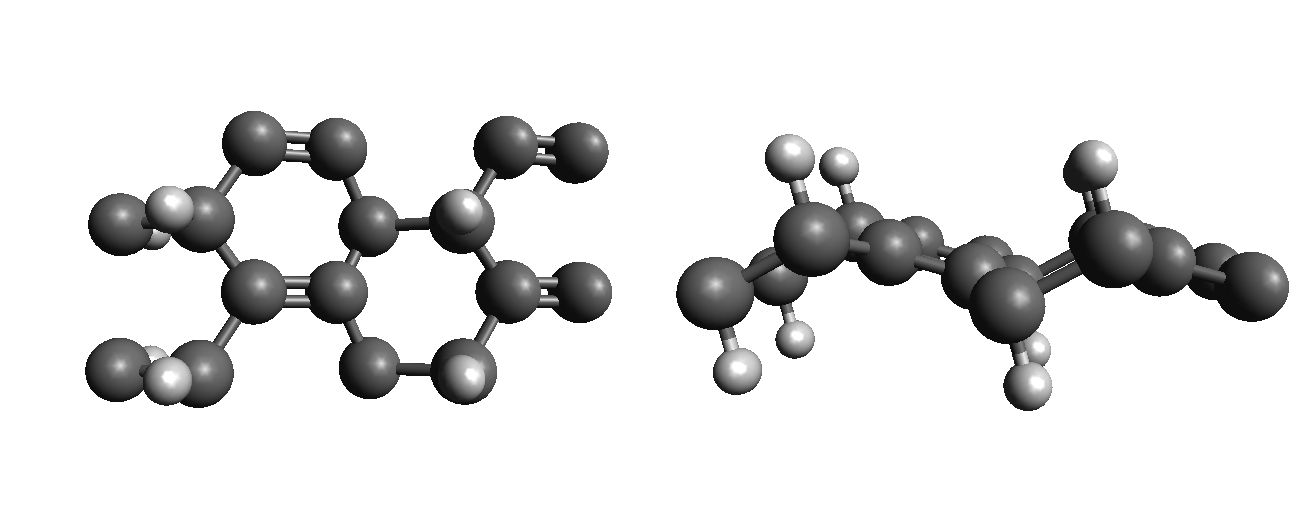
\includegraphics[width=\lw]{alt/altstruct1}}
\subfigure[\ \label{fig:upstruct}]{
    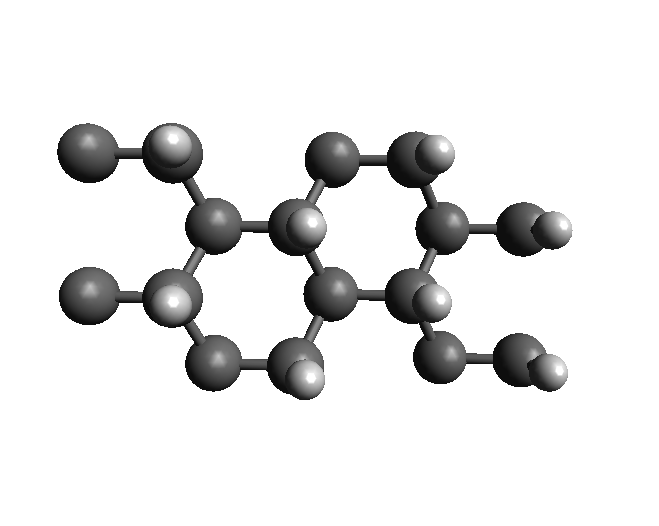
\includegraphics[width=\lw]{up/upstruct1}}
\caption{Top and side views of the [\ref{fig:altstruct}] {\altstc} and [\ref{fig:upstruct}] {\upstc} structures. The dark and light spheres correspond to carbon and hydrogen atoms, respectively.}\label{fig:structures}
\end{figure}
%%%% end figure of structures

    \subsection{Optical spin injection}

The injection and detection of spin polarized electrons into nonmagnetic materials is the core of spintronics \cite{vzutic2004spintronics,fert2008nobel,pezzoli2012optical,bottegoni2013experimental,bottegoni2013photoinduced} and an important problem in condensed matter. The process of optical spin injection of carriers appears when circularly polarized light \cite{dyakonov1984theory} insides in a semiconductor media promoting spin-polarized electrons from the valence to the conduction bands. This process takes place as a result of the interaction of electron spin and motion caused by the spin-orbit coupling in media. The DSP gives a quantitative value of the fraction of injected electrons into the conduction bands that are spin polarized. It can be calculated by full band structure local-density approximation (LDA) and $\textbf{k}\cdot \textbf{p}$ methods \cite{nastos2007full,cabellos2009stress}.

Mendoza and Cabellos derived the expressions for the optical spin generation suitable for surfaces and interfaces \cite{mendoza2012optical}. They used a slab approach in order to model the surface. They wrote the surface DSP along direction \emph{i} as

\begin{equation}
    D^{i}(\omega) = \frac{-2i \zeta^{ixy} (\omega)}{\hbar \left[ \xi^{xx}(\omega) + \xi^{yy}(\omega) \right] /2 } \label{eq:D^i}
\end{equation}

\noindent where $\zeta^{ixy} (\omega)$ and $\xi^{aa}(\omega)$ are the surface spin-injection rate tensor components and are diagonal components of the surface carrier generation rate tensor, respectively, and the indexes \emph{i},\emph{j},\emph{k} denote Cartesian coordinates.

In our calculation we consider a normal incidence of circularly polarized light propagating along the \emph{-z} direction,

\begin{equation*}
    \mathbf{E} (\omega) = E_{0}(\hat{x} -i \hat{y})/\sqrt{2}, 
\end{equation*}


\noindent where $E_{0}$ is the field intensity. Taking in account that there is possible to generate spin-polarized electrons, from the valence to the conduction bands, along the $\hat{i}$, $\hat{j}$, and $\hat{k}$ directions with incident light on the surface plane, the total DSP can be obtained by the relation 

\begin{equation*}
    |{D^{\text{T}}}| = \sqrt{ \left[ D^{x} \right]^{2} + \left[ D^{y} \right]^{2} + \left[ D^{z} \right]^{2} }
\end{equation*}

\noindent where the dependence in frequency, $\omega$, has been omitted.

    \subsection{Optical current injection}

The optical current injection is a second-order nonlinear effect that takes place in non-centrosymmetric structures \cite{nastos2006optical,cabellos2011optical,bhat2005excitonic,fraser1999quantum}. The photocurrent can be injected with a single optical beam and is produced by the interference of one photon-absorption processes associated with different linear polarizations of light \cite{sipe2000second}. Also called  \emph{circular photovoltaic effect} the optical current injection occurs in a non-centrosymmetric media when it is photoexcited with circularly polarized light, producing an interference effect in the excitation pathways, and resulting in an asymmetric population of the injected carriers in reciprocal space and, therefor, a photocurrent. This photocurrent phenomena has been studied in bulk semiconductors, one dimensional (1D) nanotubes \cite{mele2000coherent,kral2000photogalvanic}, and two dimensional (2D) surfaces \cite{mele2000coherent}.

In the year 2011 Cabellos and Mendoza \emph{et al.} \cite{cabellos2011optical}  derived the expression for the generation of the injection current for surfaces and interfaces. They defined the surface injection current as 

\begin{equation}
    \mathbf{\dot{J}}^{i}_{\text{inj}}(\omega) = \eta^{ijk}(\omega)E_{j}(\omega)E_{k}(\omega), \label{eq:eta}   
\end{equation}

\noindent where $\eta^{ijk}(\omega)$ is the surface injection current tensor. Thus, according to Eq. \ref{eq:eta}, a photocurrent is optically injected in the direction \emph{i} when two polarized electric fields, in the \emph{j} and \emph{k} directions, inside over a surface. For a surface system we have that {\ea} is given by \cite{cabellos2011optical, arzate2014optical} 

\begin{equation}
    \eta^{ijk} (\omega) = \ell_{\text{eff}} \times \sum_{\ell=1}^{n_{eff}} \eta_{ijk} (\ell|\omega). \label{eq:etaeff}
\end{equation}

\noindent where the sum is made over the number of layers that contributes to the response of the media, $\eta_{ijk} (\ell|\omega)$ corresponds to the $\ell_{\text{th}}$-layer contribution to the surface injection current tensor and $\ell_{\text{eff}}$ is the thickness to the total layers that contribute to the response. The tensor $\eta^{ijk}(\omega)$ is purely imaginary and has the property of being antisymmetric in the last two Cartesian indices, \emph{j} and \emph{k} \cite{sipe2000second,nastos2006optical}. 

Taking in account that with circularly polarized light it is possible to generate current injection along the $\hat{i}$, $\hat{j}$, and $\hat{k}$ directions with incident light on the surface plane, the total injection current can be obtained in a similar way as has been done in \ref{eq:D^i}

\begin{equation*}
    |{\eta^{\text{T}}}| = \sqrt{ \left[ \eta^{xxy} \right]^{2} + \left[ \eta^{yxy} \right]^{2} + \left[ \eta^{zxy} \right]^{2} }
\end{equation*}

\noindent where the dependence in frequency, $\omega$, has been omitted again.

The units of both $\mathbf{\dot{J}}^{i}_{\text{inj}}(\omega)$ and $\eta^{ijk} (\omega)$  are those of their bulk equivalents times $\ell_{\text{eff}}$ expressed in the corresponding units to report \cite{cabellos2011optical}.



    \subsection{Second harmonic generation}

SHG, also called frequency doubling, is a particular case of the nonlinear optical process of sum of frequency in which photons of same frequency are annihilated to produce a new photon with twice frequency, energy and half of wavelength of the initial photons. This phenomena occurs when light beams from coherent sources inside over a nonlinear media that does not present inversion of symmetry \cite{bloembergen1962light,anderson2015theory,salazar2014molecular,sipe2000second}.

Recently, Anderson \emph{et al.} \cite{anderson2015theory} developed a new formalism to calculate the second order susceptibility which includes the scissors correction, needed to have the correct value of the energy band gap; the contribution of the nonlocal part of the pseudopotentials, routinely used in ab initio band-structure calculations; and the derivation for the inclusion of the cut function, used to extract the surface response. According to that we have the expressions for the imaginary part of the interband contributions (\emph{i}) and intraband (\emph{e}) for $1\omega$ and $2\omega$

\begin{subequations}\label{eq:chis}
    \begin{equation}
        \mathrm{Im}[\chi^{\mathrm{a}\mathrm{b}\mathrm{c}}_{e,\omega}]= 
        \frac{\pi |e|^3}{2\hbar^2}
        \int \frac{dk^3}{8\pi^3}
        \sum_{vc}\sum_{q\neq(v,c)}\frac{1}{\omega^\Sigma_{cv}}
        \left[
        \frac{\mathrm{Im}[\mathcal{V}^{\Sigma,\mathrm{a}}_{qc}\{r^{\mathrm{b}}_{cv}r^{\mathrm{c}}_{vq}\}]}
        {(2\omega^\Sigma_{cv}-\omega^\Sigma_{cq})} 
        -\frac{\mathrm{Im}[\mathcal{V}^{\Sigma,\mathrm{a}}_{vq}\{r^{\mathrm{c}}_{qc}r^{\mathrm{b}}_{cv}\}]}
        {(2\omega^\Sigma_{cv}-\omega^\Sigma_{qv})}
        \right]\delta(\omega^\Sigma_{cv}-\omega),
    \end{equation}  
    \begin{equation}
        \mathrm{Im}[\chi^{\mathrm{a}\mathrm{b}\mathrm{c}}_{i,\omega}]= 
        \frac{\pi\vert e\vert^3}{2\hbar^2}
        \int \frac{dk^3}{8\pi^3}
        \sum_{cv}\frac{1}{(\omega^\Sigma_{cv})^{2}}
        \left[
        \mathrm{Re}\left[\left\{r^{\mathrm{b}}_{cv}\left(\mathcal{V}^{\Sigma,\mathrm{a}}_{vc}\right)_{;k^{\mathrm{c}}}\right\}\right]
        +\frac{\mathrm{Re}\left[\mathcal{V}^{\Sigma,\mathrm{a}}_{vc}\left\{r^{\mathrm{b}}_{cv}
        \Delta^{\mathrm{c}}_{cv}\right\}\right]}{\omega^\Sigma_{cv}} 
        \right]\delta(\omega^\Sigma_{cv}-\omega),
    \end{equation}
    \begin{equation}
        \mathrm{Im}[\chi^{\mathrm{a}\mathrm{b}\mathrm{c}}_{e,2\omega}]= 
        -\frac{\pi |e|^3}{2\hbar^2}
        \int \frac{dk^3}{8\pi^3}
        \sum_{vc}\frac{4}{\omega^\Sigma_{cv}}
        \left[
        \sum_{v'\ne
          v}\frac{\mathrm{Im}[\mathcal{V}^{\Sigma,\mathrm{a}}_{vc}\{r^{\mathrm{b}}_{cv'}r^{\mathrm{c}}_{v'v}\}]}
        {2\omega^\Sigma_{cv'}-\omega^\Sigma_{cv}}
        - \sum_{c'\ne
          c}\frac{\mathrm{Im}[\mathcal{V}^{\Sigma,\mathrm{a}}_{vc}\{r^{\mathrm{c}}_{cc'}r^{\mathrm{b}}_{c'v}\}]}
        {2\omega^\Sigma_{c'v}-\omega^\Sigma_{cv}}
        \right]\delta(\omega^\Sigma_{cv}-2\omega),
    \end{equation}
    \begin{equation}
        \mathrm{Im}[\chi^{\mathrm{a}\mathrm{b}\mathrm{c}}_{i,2\omega}]= 
         \frac{\pi \vert
           e\vert^{3}}{2\hbar^2}
        \int \frac{dk^3}{8\pi^3}
        \sum_{vc}\frac{4}{(\omega^\Sigma_{cv})^{2}}
        \left[\mathrm{Re}\left[\mathcal{V}^{\Sigma,\mathrm{a}}_{vc}\left\{\left(r^{\mathrm{b}}_{cv}\right)_{;k^{\mathrm{c}}}
        \right\}\right] -
        \frac{2\mathrm{Re}\left[\mathcal{V}^{\Sigma,\mathrm{a}}_{vc}\left\{r^{\mathrm{b}}_{cv}
        \Delta^{\mathrm{c}}_{cv}\right\}\right]}{\omega^\Sigma_{cv}}\right]\delta(\omega^\Sigma_{cv}-2\omega)
        .
    \end{equation}
\end{subequations}

\noindent Here, the factor of 2 for spin degeneracy is not included and the real part of each contribution can be obtained through a Kramers-Kronig transformation \cite{tancogne2014effect} and 

\begin{equation}\label{eq:chitotal}
    \chi^{abc} = \chi^{abc}_{e,\omega} + \chi^{abc}_{e,2\omega} + \chi^{abc}_{i,\omega} + \chi^{abc}_{i,2\omega}
    .
\end{equation}

As made before, in Eq. \ref{eq:chis} and \ref{eq:chitotal} the dependence in frequency, $\omega$, has been omitted. For our case in Eq. \ref{eq:chis}, the  expression $\mathcal{V}^{\Sigma}$ corresponds to the sum of the LDA and non-local velocity matrix elements, $r^{\mathrm{a}} $ are the position matrix elements and $\Delta^{a}_{nm} = v^{\text{LDA},a}_{nn} - v^{\text{LDA},a}_{mm} $ \cite{anderson2015theory}. To accomplish the required intrinsic permutation symmetry, the \{\} notation symmetrizes the $bc$ Cartesian indices, i.e., $\{u^{b}s^{c}\} = (u^{b}s^{c} + u^{c}s^{b})/{2}$ and so, $\chi^{abc} = \chi^{acb}$. The units of $\chi^{ijk} $, again, are those of their bulk equivalents times $\ell_{\text{eff}}$ expressed in the corresponding units to report.



%%               end of theory section                 %%
%%                                                     %%
%%%%%%%%%%%%%%%%%%%%%%%%%%%%%%%%%%%%%%%%%%%%%%%%%%%%%%%%%
%%%%%%%%%%%%%%%%%%%%%%%%%%%%%%%%%%%%%%%%%%%%%%%%%%%%%%%%%


%%%%%%%%%%%%%%%%%%%%%%%%%%%%%%%%%%%%%%%%%%%%%%%%%%%%%%%%%
%%%%%%%%%%%%%%%%%%%%%%%%%%%%%%%%%%%%%%%%%%%%%%%%%%%%%%%%%
%%               begin of results section              %%
%%                                                     %%


\section{Results} % (fold)
\label{sec:results}

% section results (end)

We present the results of the numerical calculations for \da, \ea, and SHG for the hydrogenated graphene structures, {\altstc} and {\upstc} shown in Fig. \ref{fig:structures}. Both structures are infinite carbon planes in an hexagonal honeycomb lattice with \%50 of hydrogenation in two different arrangements: the \emph{alt} structure [Fig \ref{fig:altstruct}] has alternating hydrogen bonds in the top and bottom sides of the carbon plane; the \emph{up} structure [Fig \ref{fig:upstruct}] has hydrogen bonds only in the top side. Both structures are non-centrosymmetric and has a thickness of 5.56 and 2.76 Angstroms, respectively. A vacuum length at least  five times the thickness for each structure was taken to construct the super-cell.  

For this work we used the ABINIT code \cite{torrent2008implementation} for the calculation of the self-consistent ground state and their Kohn-Sham states using DFT--LDA in the plane waves approximation. Also we used the relativistic separable dual-space Gaussian pseudopotentials of Hartwigsen-Goedecker-Hutter (HGH) \cite{hartwigsen1998relativistic} including the spin-orbit interaction, necessary to make the calculations of $D^{i} $ but not in the cases of \ea and SHG. Moreover, we have taken a cutoff energy of 65 and 40\,Ha for the \emph{alt} and \emph{up} structures, respectively, and the energy eigenvalues and matrix elements were calculated using 14452 and 8452 \textbf{k}\,points in the irreducible BZ.

In Figs. \ref{fig:alt-Da} and \ref{fig:up-Da} we show the spectra obtained for {\da} of the {\altstc} and {\upstc} structures, respectively. Values over (under) zero define a positive (negative) direction of spin polarization along the \emph{a} direction. It can be observed that for both structures we have more than 40\% of {\da} and a maximum absolute value in the \emph{y} direction, reaching almost a 50\% in the \emph{alt} structure. In table \ref{tab:dacomp} we show a comparison of the maximum degree of spin polarization reported for different structures.



%%%% begin table comparison Da
\begin{table}[h]
    \caption{Comparison of the reported absolute values for the highest percentage of {\da} for different structures. ($^{*}$This work.)}
    \label{tab:dacomp}
    \centering
    \begin{ruledtabular}
    \begin{tabular}{lccc}
    Structure & Energy & {\da} &  Reference\\
              & [eV]   & \emph{a}, [\%] \\
    \hline
    {\altstc}                  & 0.719 & y, 48 & *     \\
    {\upstc}                   & 0.40  & y, 42 & *     \\
    Si(111)-In $8\times2$   & 0.74  & z, 32 & \cite{arzate2014optical}  \\
    Si(111)-As $1\times1$   & 2.20  & z, 100& \cite{mendoza2012optical} \\
    Bulk Si                 & 3.44  & z, 30 & \cite{nastos2007full}     \\
    \end{tabular}
    \end{ruledtabular}

\end{table}
%%%% end table comparison Da


To report the {\ea} we took in account that our structures are infinite carbon-hydrogen layers. So in Eq. \ref{eq:etaeff} we defined the $\ell_{\text{eff}}$ as the thickness of each structure, 5.56 and 2.76 Angstroms for the \emph{alt} and \emph{up} structures.

We show in Figs. \ref{fig:alt-eta} and \ref{fig:up-eta}  the spectra obtained for the current tensor {\ea} of the structures \emph{alt} and \emph{up}, respectively. We can observe that circularly polarized light on the plane $xy$ produces injection current along three directions. Values over (under) zero define a positive (negative) direction of current injection along the \emph{a} direction. From Fig. \ref{fig:eta} we can see that for the \emph{alt} structure spectra [Fig. \ref{fig:alt-eta}] we have a positive maximum in the \emph{y} direction for an incident beam energy of 1.25\,eV, reaching a value of 3.7\,mC$^{3}$/J$^{2}$s$^{2}$ . Also, for the \emph{up} structure spectra [Fig. \ref{fig:up-eta}] we have a negative maximum in the \emph{x} direction for an incident beam energy of 0.405\,eV, reaching a value of 3.5\,mC$^{3}$/J$^{2}$s$^{2}$. In table \ref{tab:etacomp} we present a comparison of the maximum current injection reported for different structures.


%%%% begin figure Da
\begin{figure}[h!]
    \centering
    \subfigure[\ \label{fig:alt-Da}]{
        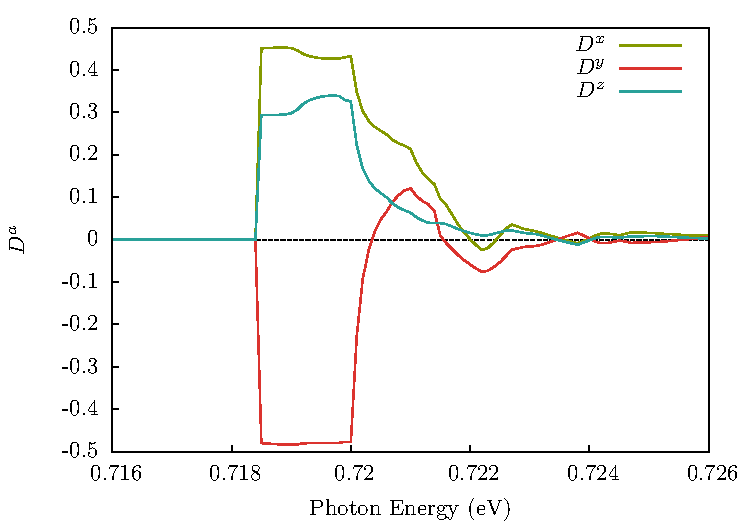
\includegraphics[width=\lw]{alt/alt-Da-final}}
    \subfigure[\ \label{fig:up-Da}]{
        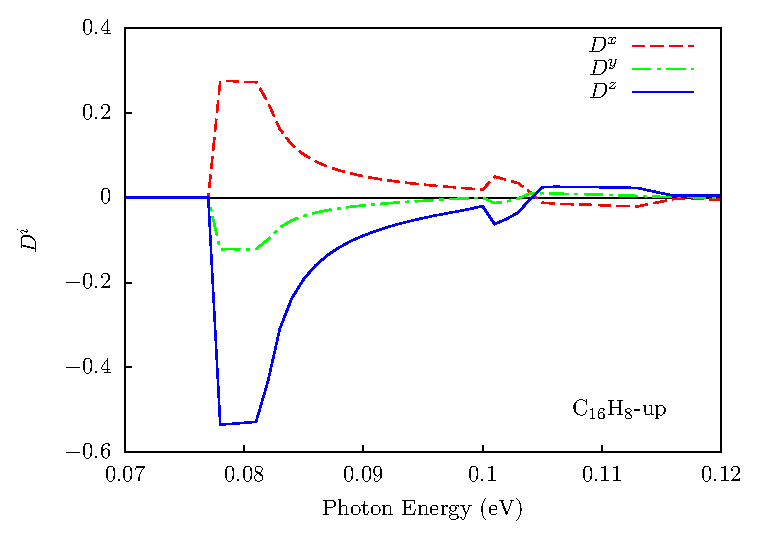
\includegraphics[width=\lw]{up/up-Da-final}}
    \caption{(Color online) Spectra of the degree of spin polarization along the direction \emph{i}, {\da}, for the hydrogenated graphene structures {\altstc} [Fig. \ref{fig:alt-Da}] and {\upstc} [Fig. \ref{fig:up-Da}] under incidence of circularly polarized light.}\label{fig:Da}
\end{figure}
%%%% end figure Da



%%%% begin table comparison eta
\begin{table}[]
    \caption{Comparison of the highest reported absolute values of {\ea} for different structures. ($^{*}$This work.)}
    \label{tab:etacomp}
    \centering
    \begin{ruledtabular}
    \begin{tabular}{lccc}
    Structure & Energy &{\ea} &  Ref.\\
              & [eV]   & \hspace{-2.5mm} \emph{a},\, [mC$^{3}$/J$^{2}$s$^{2}$] \\
    \hline
    {\altstc}               & 1.25  & y, 3.70  & *     \\
    {\upstc}                & 0.405 & x, 3.50  & *     \\
    Si(111)-In $8\times2$   & 1.24  & y, 0.35  & \cite{arzate2014optical}  \\
    Si(111) $2\times1$      & 0.75  & y, 1.22  & \cite{mendoza2012optical} \\
    GaAs(110) clean         & 4.30  & y, 0.30  & \cite{nastos2007full}     \\
    \end{tabular}
    \end{ruledtabular}
\end{table}
%%%% end table comparison eta


%%%% begin figure eta
\begin{figure}[h!]
    \centering
    \subfigure[\ \label{fig:alt-eta}]{
            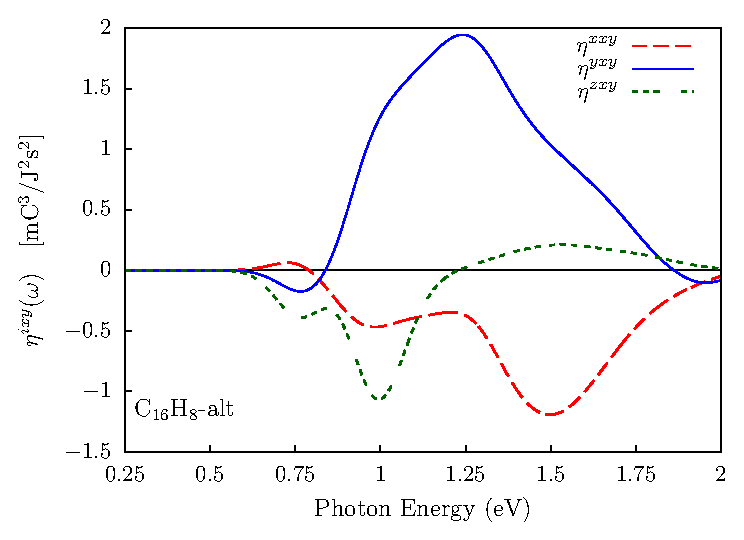
\includegraphics[width=\lw]{alt/alt-eta_sm-final}}
    \subfigure[\ \label{fig:up-eta}]{
            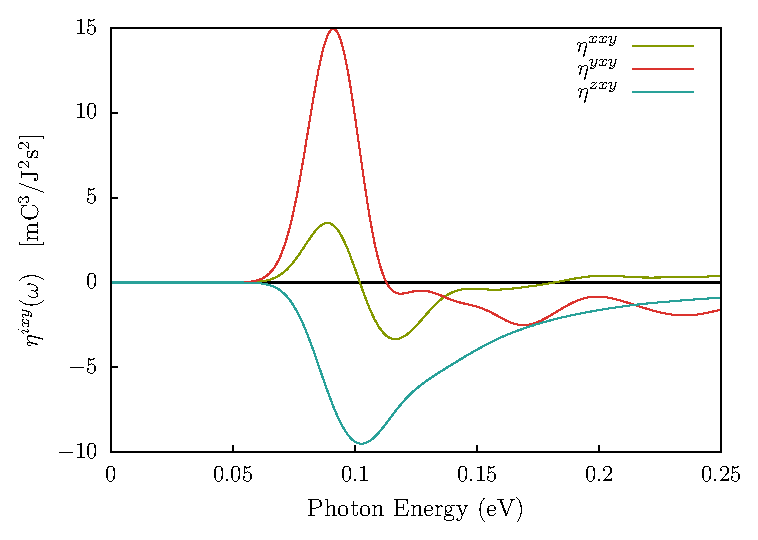
\includegraphics[width=\lw]{up/up_eta_sm_final}}
    \caption{(Color online) Spectra of the injection current tensor along the direction \emph{i}, {\ea}, for the hydrogenated graphene structures {\altstc} [Fig \ref{fig:alt-eta}] and {\upstc} [Fig. \ref{fig:up-eta}] under incidence of circularly polarized light.}\label{fig:eta}
\end{figure}
%%%% end figure eta


%%%% begin figure shg alt
\begin{figure}[h!]
    \centering
    \subfigure[\ \label{fig:alt-shg-abs}]{
            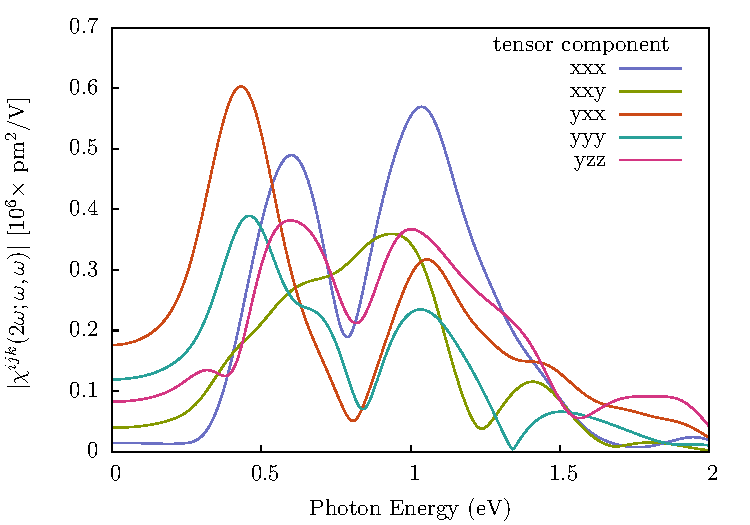
\includegraphics[width=\lw]{alt/alt_shg_final-abs_sm}}
    \subfigure[\ \label{fig:alt-shg-im}]{
            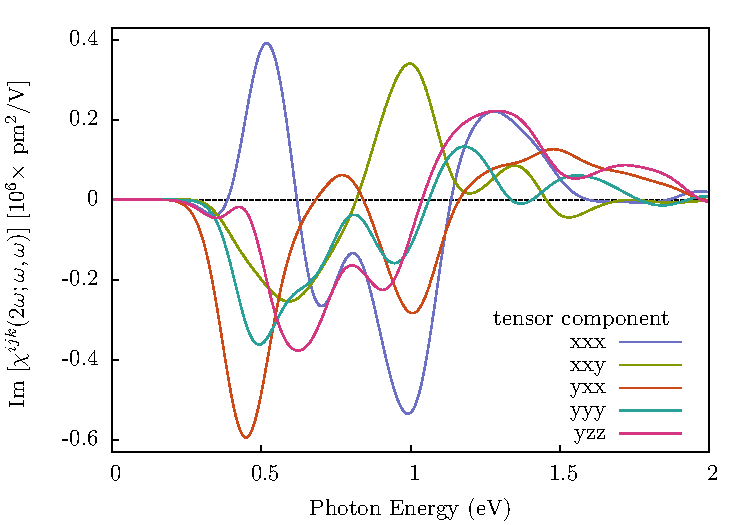
\includegraphics[width=\lw]{alt/alt_shg_final-im_sm}}
    \subfigure[\ \label{fig:alt-shg-re}]{
            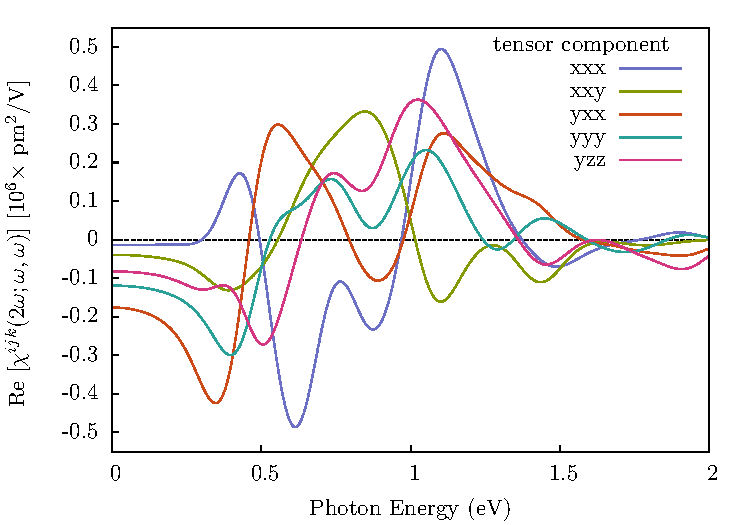
\includegraphics[width=\lw]{alt/alt_shg_final-re_sm}}
    \caption{(Color online) Spectra of the SHG for the {\altstc}. The Fig. [\ref{fig:alt-shg-abs}] corresponds to the absolute value for the non zero components {\huge Something else}.}\label{fig:shg-alt}
\end{figure}
%%%% end figure shg alt



%%%% begin figure shg up
\begin{figure}[h!]
    \centering
    \subfigure[\ \label{fig:up-shg-abs}]{
            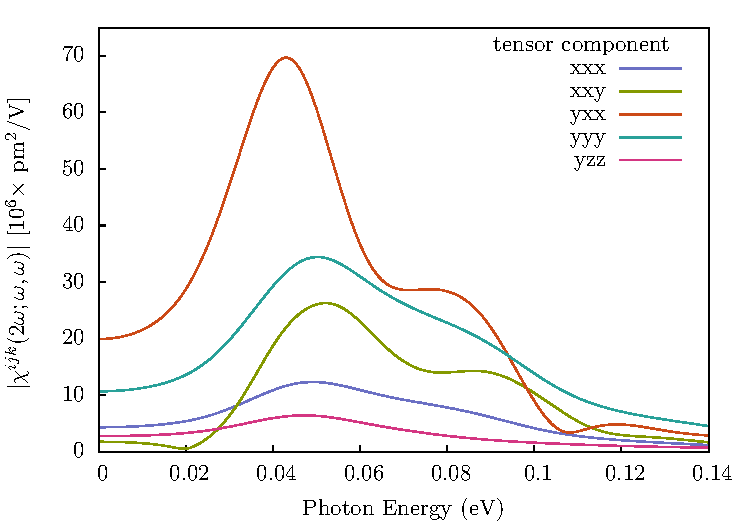
\includegraphics[width=\lw]{up/up_shg_final_abs_sm}}
    \subfigure[\ \label{fig:up-shg-im}]{
            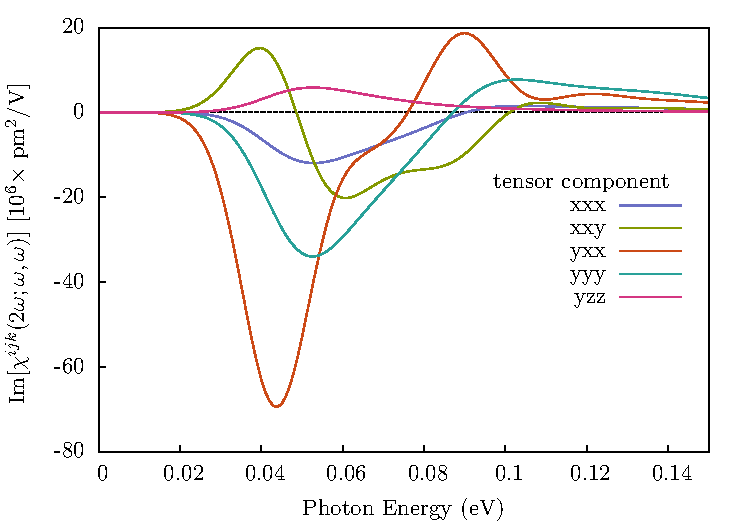
\includegraphics[width=\lw]{up/up_shg_final_im-sm}}
    \subfigure[\ \label{fig:up-shg-re}]{
            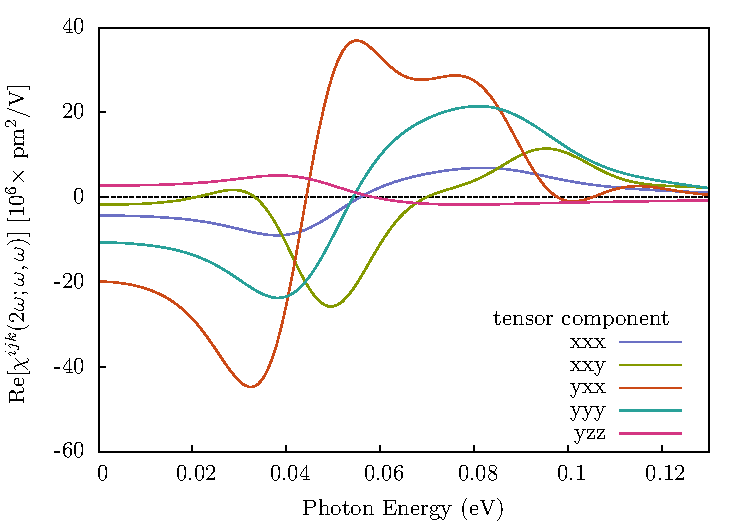
\includegraphics[width=\lw]{up/up_shg_final_re-sm}}
    \caption{(Color online) Spectra of the SHG for the {\upstc}. The Fig. [\ref{fig:up-shg-abs}] corresponds to the absolute value for the non zero components {\huge Something else}.}\label{fig:shg-up}
\end{figure}
%%%% end figure shg up



%%%                                                    %%
%%               end of results section                %%
%%%%%%%%%%%%%%%%%%%%%%%%%%%%%%%%%%%%%%%%%%%%%%%%%%%%%%%%%
%%%%%%%%%%%%%%%%%%%%%%%%%%%%%%%%%%%%%%%%%%%%%%%%%%%%%%%%%


%%%%%%%%%%%%%%%%%%%%%%%%%%%%%%%%%%%%%%%%%%%%%%%%%%%%%%%%%
%%%%%%%%%%%%%%%%%%%%%%%%%%%%%%%%%%%%%%%%%%%%%%%%%%%%%%%%%
%%               begin of conclusions section          %%
%%                                                     %%

\section{Conclusions} % (fold)
\label{sec:conclusions}


%%                                                     %%
%%             end of conclusions section              %%
%%%%%%%%%%%%%%%%%%%%%%%%%%%%%%%%%%%%%%%%%%%%%%%%%%%%%%%%%
%%%%%%%%%%%%%%%%%%%%%%%%%%%%%%%%%%%%%%%%%%%%%%%%%%%%%%%%%

%%%%%%%%%%%%%%%%%%%%%%%%%%%%%%%%%%%%%%%%%%%%%%%%%%%%%%%%%
%%%%%%%%%%%%%%%%%%%%%%%%%%%%%%%%%%%%%%%%%%%%%%%%%%%%%%%%%
%%               begin of Acknowledgment section          %%
%%                                                     %%

\section{Acknowledgment} % (fold)
\label{sec:Acknouledgment}


%%                                                     %%
%%             end of Acknowledgment section              %%
%%%%%%%%%%%%%%%%%%%%%%%%%%%%%%%%%%%%%%%%%%%%%%%%%%%%%%%%%
%%%%%%%%%%%%%%%%%%%%%%%%%%%%%%%%%%%%%%%%%%%%%%%%%%%%%%%%%


% \begin{thebibliography}{37}
\bibliography{graphene_structures}
% \bibliographystyle{apsrev.bst}
% \end{thebibliography}

\end{document}